\documentclass[]{bytedance_seed}

% single-column: \documentclass[]{bytedance_seed}, 
%Please prioritize using single-column。

% twocolumn: \documentclass[twocolumn]{bytedance_seed}

\usepackage[toc,page,header]{appendix}


%%%%%%%%%%%%%%%%%%%%%%%%%%%%%%%%%%%%

\usepackage{minitoc}
\usepackage{cleveref} 
\usepackage{subcaption}
\usepackage{booktabs}

\usepackage{natbib}
% Standard package includes
% \usepackage{times}
\usepackage{latexsym}

% For proper rendering and hyphenation of words containing Latin characters (including in bib files)
% \usepackage[T1]{fontenc}
% For Vietnamese characters
% \usepackage[T5]{fontenc}
% See https://www.latex-project.org/help/documentation/encguide.pdf for other character sets
\usepackage{url}
\usepackage{amssymb}
\usepackage[utf8]{inputenc}
\usepackage{microtype}
\usepackage{booktabs}
\usepackage{pifont} 
\usepackage{multirow}
\usepackage{makecell}
\usepackage{paralist}
\usepackage{xspace}
\usepackage{color}
\usepackage{xcolor}
\usepackage{colortbl}
\usepackage{adjustbox}
\usepackage{hyperref} 
\usepackage[edges]{forest}
\usepackage{tikz} 
% \usepackage{longtable} % For tables that can span multiple pages
\usepackage{caption}
\usepackage{amsfonts}

\hypersetup{
    colorlinks,
    linkcolor={blue!80!black},
    citecolor={blue!80!black},
    % urlcolor={brown!50!black}
}
\tikzset{
    root/.style =             {align=center, text width=1cm, rounded corners=3pt, line width=0.3mm, fill=gray!10, draw=gray!80, font=\small},
    % demographic 
    demographic/.style =         {align=center, text width=1.8cm, rounded corners=3pt, line width=0.3mm, fill=blue!10, draw=blue!80, font=\footnotesize},
    demographic_work/.style =    {align=center, text width=10cm, rounded corners=3pt, line width=0.3mm, fill=blue!10, draw=blue!0, font=\footnotesize},
    % character 
    character/.style =         {align=center, text width=1.8cm, rounded corners=3pt, line width=0.3mm, fill=red!10, draw=red!80, font=\footnotesize},
    character_work/.style =    {align=center, text width=10cm, rounded corners=3pt, line width=0.3mm, fill=red!10, draw=red!0, font=\footnotesize},
    % Personalization
    personalization/.style =           {align=center, text width=1.8cm, rounded corners=3pt, line width=0.3mm, fill=cyan!10, draw=cyan!80, font=\footnotesize},
    personalization_work/.style =      {align=center, text width=10cm, rounded corners=3pt, line width=0.3mm, fill=cyan!10, draw=cyan!0, font=\footnotesize},
    % risks
    risk/.style =         {align=center, text width=1.8cm, rounded corners=3pt, line width=0.3mm, fill=orange!10, draw=orange!80, font=\footnotesize},
    risk_work/.style =    {align=center, text width=10cm, rounded corners=3pt, line width=0.3mm, fill=orange!10, draw=orange!0, font=\footnotesize},
}

% If the title and author information does not fit in the area allocated, uncomment the following
%
% \setlength\titlebox{7cm}
%
% and set <dim> to something 5cm or larger.
\newcommand{\new}[1]{\textcolor{purple}{{#1}}}
\newcommand{\todo}[1]{\textcolor{red}{{[$\blacksquare$ TODO: #1]}}}
\newcommand{\method}{\textsc{\textbf{DAPO}}\xspace}
\newcommand{\ie}{\textit{i.e.}\xspace}
\newcommand{\eg}{\textit{e.g.}\xspace}
\newcommand{\wo}{\textit{w/o}\xspace}
\newcommand{\dq}[1]{``#1''}
\newcommand{\sq}[1]{`#1'}
\newcommand{\cjj}[1]{\textcolor{red}{{[cjj: #1]}}}
\newcommand{\jj}[1]{\textcolor{cyan}{\small{\bf [JJ: #1]}}}
\newcommand{\qiying}[1]{\textcolor{purple}{{[qiying: #1]}}}
\newcommand{\hao}[1]{\textcolor{blue}{{[hao: #1]}}}
\newcommand{\zheng}[1]{\textcolor{brown}{{[zheng: #1]}}}
\newcommand{\hongli}[1]{\textcolor{teal}{{[hongli: #1]}}}
\newcommand{\weinan}[1]{\textcolor{orange}{{[weinan: #1]}}}


\newcommand{\etc}{\textit{etc}\xspace}
\newcommand{\cmark}{\ding{51}}
\newcommand{\xmark}{\ding{55}}
\newcommand{\customcite}[2]{\hyperlink{cite.#2}{#1}}

% \setlength\tabcolsep{3.5pt}

\newcommand\footnoteplain[1]{%
  \begingroup
  \renewcommand\thefootnote{}\footnote{#1}%
  \addtocounter{footnote}{-1}%
  \endgroup
}

\usepackage{CJK}
% \pagestyle{plain} % very strange, fixes page number centering problem.


%%%%%%%%%%%%%%%%%%%%

\title{DAPO: An Open-Source LLM Reinforcement Learning System at Scale}
% Democratizing LLM Reasoning \\ by Unveiling the Secrets of RL Scaling}
% Open-Source LLM RL System Surpassing DeepSeek's RL}
% Democratizing LLM Reasoning \\ by Unveiling the Secrets of RL Scaling}

% 

% \author[1,2,*, \dagger]{Author1}
% \author[1]{Author2}
% \author[1,2,*]{Author3}
% \author[1]{Author4}
% \author[1, \dagger]{Author5}

%论文单位请使用ByteDance Seed

\affiliation[1]{ByteDance Seed\quad $^2$Institute for AI Industry Research (AIR), Tsinghua University}
% \affiliation[2]{}
\affiliation[3]{The University of Hong Kong}
\affiliation[4]{SIA-Lab of Tsinghua AIR and ByteDance Seed}



\contribution{Full author list in Contributions}
% \contribution[*]{Work done at ByteDance Seed}
% \contribution[\dagger]{Corresponding authors}

\abstract{

Inference scaling empowers LLMs with unprecedented reasoning ability, with reinforcement learning as the core technique to elicit complex reasoning. However, key technical details of state-of-the-art reasoning LLMs are concealed (such as in OpenAI o1 blog and DeepSeek R1 technical report), thus the community still struggles to reproduce their RL training results.
We propose the \textbf{D}ecoupled Clip and \textbf{D}ynamic s\textbf{A}mpling \textbf{P}olicy \textbf{O}ptimization (\method) algorithm, and fully open-source a state-of-the-art large-scale RL system that achieves 50 points on AIME 2024 using Qwen2.5-32B base model.
Unlike previous works that withhold training details, we introduce four key techniques of our algorithm that make large-scale LLM RL a success. In addition, we open-source our training code, which is built on the \textbf{verl} framework~\footnote{\url{https://github.com/volcengine/verl}}, along with a carefully curated and processed dataset. These components of our open-source system enhance reproducibility and support future research in large-scale LLM RL.

}

% March 17, 2025
% \today

\date{March 17, 2025}
\correspondence{Qiying Yu at \email{yuqy22@mails.tsinghua.edu.cn}}

% You can add additional info fields as follows 
\checkdata[Project Page]{\url{https://dapo-sia.github.io/}}

\begin{document}

\maketitle

%不需要目录就注释掉 注意目录不要和第一页放在一块 要有\newpage
%\newpage
%\tableofcontents
%\newpage

% \qiying{Comment like this}

% \hao{Comment like this}

% \zheng{Comment like this}

% \weinan{Comment like this}

% \hongli{Comment like this}
\vspace{-20pt}
\begin{figure}[h]
    \centering
    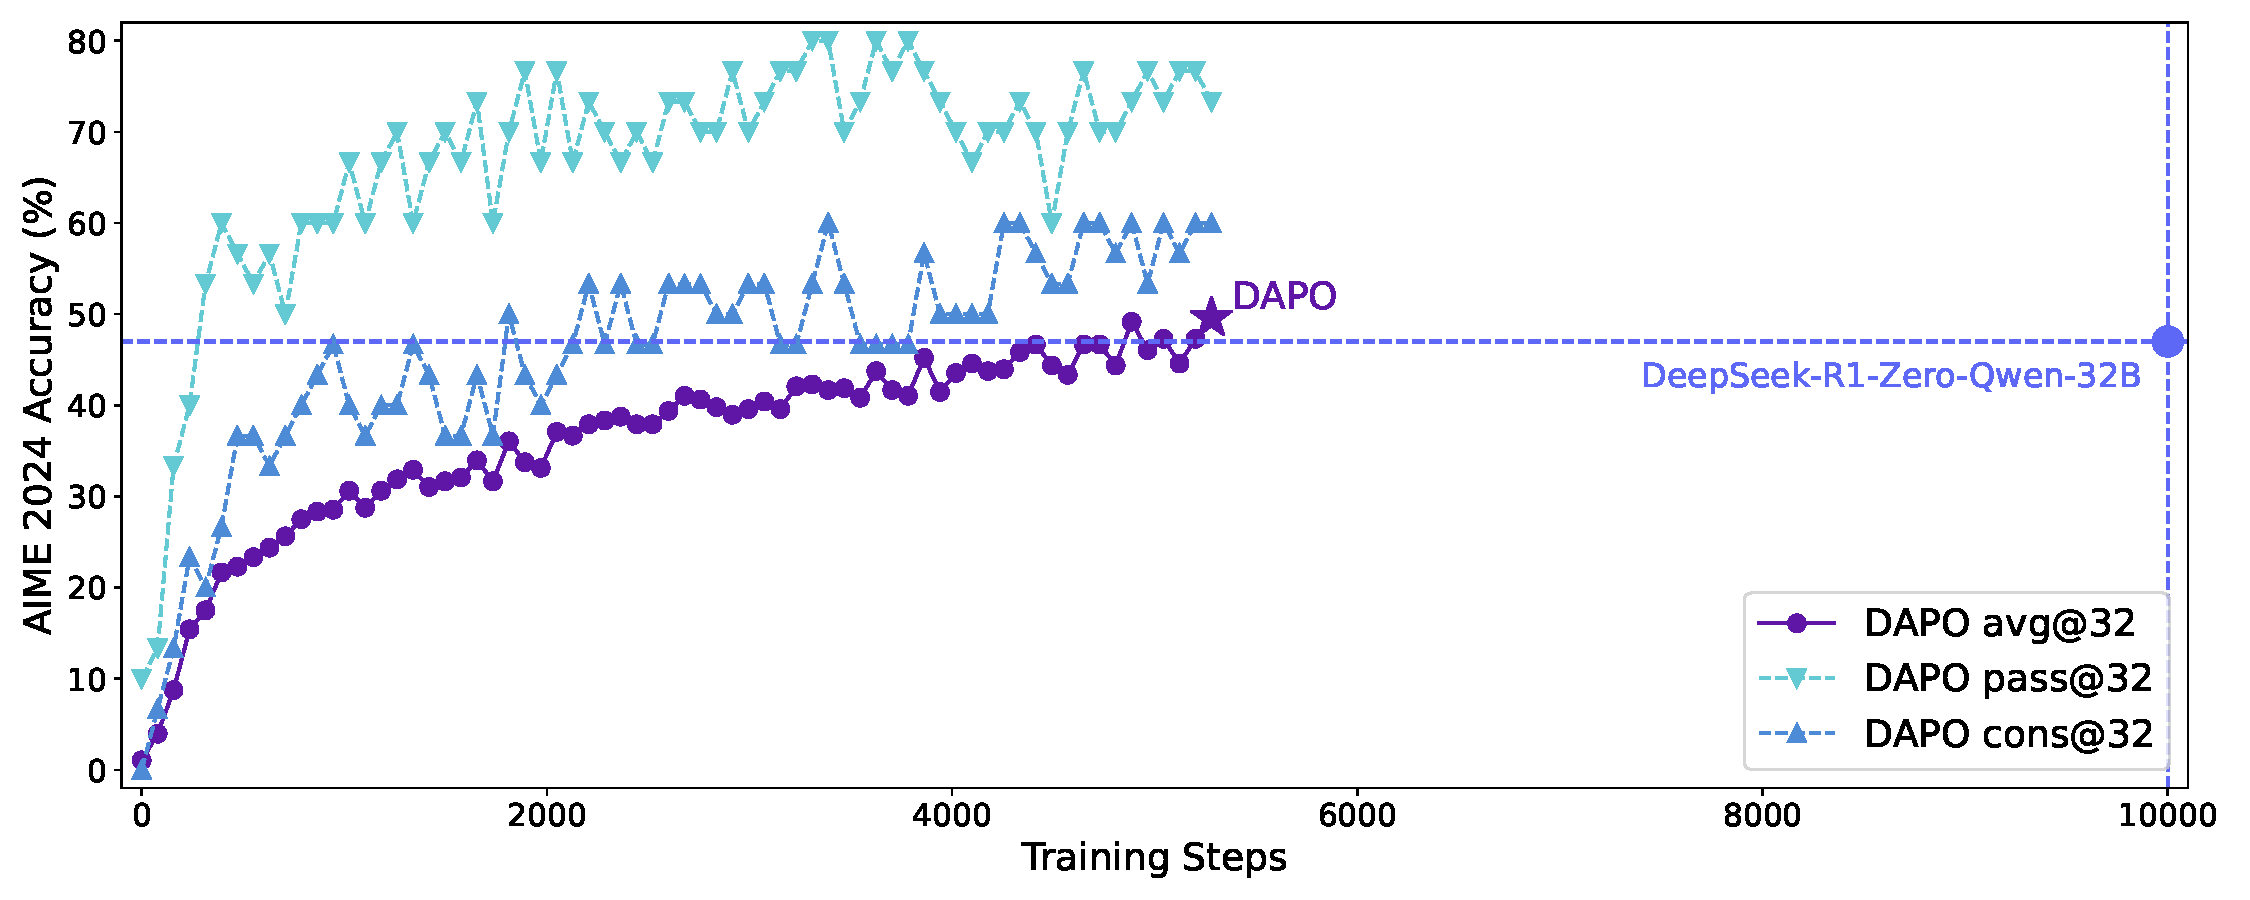
\includegraphics[width=0.92\linewidth]{figures/score.pdf}
    \caption{AIME 2024 scores of \method on the Qwen2.5-32B base model, outperforming the previous SoTA DeepSeek-R1-Zero-Qwen-32B using 50\% training steps.}
    \label{fig:front}
\end{figure}

\newpage
\section{Introduction}

Test-time scaling such as OpenAI's o1~\cite{o1} and DeepSeek's R1~\cite{guo2025deepseek} brings a profound paradigm shift to Large Language Models (LLMs)~\cite{gpt4,claude35sonnet,gpt3,chowdhery2023palm,dsv3}. Test-time scaling enables longer Chain-of-Thought thinking and induces sophisticated reasoning behaviors, which makes the models superior in competitive math and coding tasks like AIME and Codeforces.

The central technique driving the revolution is large-scale Reinforcement Learning (RL), which elicits complex reasoning behaviors such as self-verification and iterative refinement. However, the actual algorithm and key recipe for scalable RL training remains a myth, hidden from technical reports of existing reasoning models~\cite{o1,guo2025deepseek,grok,gemini-thinking,qwq,k1.5}. In this paper, we reveal significant obstacles in large-scale RL training and open-source a scalable RL system with fully open-sourced algorithm, training code and dataset that provides democratized solutions with industry-level RL results. 

We experiment over Qwen2.5-32B~\cite{yang2024qwen2} as the pretrained model for RL. In our initial GRPO run, we achieved only 30 points on AIME — a performance significantly below DeepSeek’s RL (47 points). A thorough analysis reveals that the naive GRPO baseline suffers from several key issues such as entropy collapse, reward noise, and training instability. The broader community has encountered similar challenges in reproducing DeepSeek's results~\cite{rendarl,OpenReasonerZero2025,hu2025reinforce++,cui2025process,lee2024token,kazemnejad2024vineppo,yuan2025s} suggesting that critical training details may have been omitted in the R1 paper that are required to develop an industry-level, large-scale, and reproducible RL system.

To close this gap, we release an open-source state-of-the-art system for large-scale LLM RL, which achieves 50 points on AIME 2024 based on Qwen2.5-32B model, outperforming previous state-of-the-art results achieved by DeepSeek-R1-Zero-Qwen-32B~\cite{guo2025deepseek} (47 points) using 50\% training steps (Figure~\ref{fig:front}). We propose the \textbf{D}ecoupled Clip and \textbf{D}ynamic s\textbf{A}mpling \textbf{P}olicy \textbf{O}ptimization (\textbf{DAPO}) algorithm, and introduce 4 key techniques to make RL shine in the long-CoT RL scenario. Details are presented in Section~\ref{sec:method}.
\begin{enumerate}
    \item \textbf{Clip-Higher}, which promotes the diversity of the system and avoids entropy collapse;
    \item \textbf{Dynamic Sampling}, which improves training efficiency and stability;
    \item \textbf{Token-Level Policy Gradient Loss}, which is critical in long-CoT RL scenarios;
    \item \textbf{Overlong Reward Shaping}, which reduces reward noise and stabilizes training.
\end{enumerate}
Our implementation is based on verl~\cite{sheng2024hybridflow}. By fully releasing our state-of-the-art RL system including training code and data, we aim to reveal valuable insights to large-scale LLM RL that benefit the larger community.

\section{Preliminary}

\subsection{Proximal Policy Optimization (PPO)}
PPO~\cite{schulman2017proximal} introduces a clipped surrogate objective for policy optimization. By constraining the policy updates within a proximal region of the previous policy using clip, PPO stabilizes training and improves sample efficiency. Specifically, PPO updates the policy by maximizing the following objective:
\begin{equation}
\begin{aligned}
\mathcal{J}_\text{PPO}(\theta) = \mathbb{E}_{(q,a)\sim \mathcal{D},o_{\le t}\sim\pi_{\theta_{\text{old}}}(\cdot\mid q)}
\Bigg[ 
\min \Bigg( \frac{\pi_{\theta}(o_t\mid q,o_{<t})}{\pi_{\theta_{\text{old}}}(o_t\mid q,o_{<t})} \hat{A}_t,  
\ \text{clip} \Bigg( \frac{\pi_{\theta}(o_t\mid q,o_{<t})}{\pi_{\theta_{\text{old}}}(o_t\mid q,o_{<t})}, 1 - \varepsilon, 1 + \varepsilon \Bigg) \hat{A}_t \Bigg) \Bigg],
\label{eq:ppoloss}
\end{aligned}
\end{equation}
where $(q,a)$ is a question-answer pair from the data distribution $\mathcal{D}$, $\varepsilon$ is the clipping range of importance sampling ratio, and $\hat{A}_t$ is an estimator of the advantage at time step $t$. Given the value function $V$ and the reward function $R$, $\hat{A}_t$ is computed using the Generalized Advantage Estimation (GAE)~\cite{schulman2018highdimensionalcontinuouscontrolusing}:
\begin{equation}
\begin{aligned}
    &\hat{A}_t^{\text{GAE}(\gamma,\lambda)} = \sum_{l=0}^{\infty}(\gamma\lambda)^l\delta_{t+l},
\end{aligned}
\end{equation}
where
\begin{equation}
    \delta_{l}=R_l+\gamma V(s_{l+1})-V(s_l),\quad 0\le\gamma,\lambda\le1.
\end{equation}


\subsection{Group Relative Policy Optimization (GRPO)}

Compared to PPO, GRPO eliminates the value function and estimates the advantage in a group-relative manner. For a specific question-answer pair $(q,a)$, the behavior policy $\pi_{\theta_\text{old}}$ samples a group of $G$ individual responses $\{ o_i\}_{i=1}^G$. Then, the advantage of the $i$-th response is calculated by normalizing the group-level rewards $\{ R_i \}_{i=1}^G$:
\begin{equation}
\hat{A}_{i,t} = \frac{r_i - \text{mean}(\{R_i\}_{i=1}^G)}{\text{std}(\{R_i\}_{i=1}^G)}.
\end{equation}

Similar to PPO, GRPO adopts a clipped objective, together with a directly imposed KL penalty term:
% Additionally, the KL-regularization between current policy $\pi_\theta$ and the reference policy $\pi_\text{ref}$ is directly added to the loss function:
\begin{equation}
\begin{aligned}
\mathcal{J}_\text{GRPO}(\theta)& = \mathbb{E}_{(q,a)\sim \mathcal{D}, \{o_i\}_{i=1}^G\sim \pi_{\theta_\text{old}}(\cdot\mid q)} \\&
\Bigg[ \frac{1}{G}\sum_{i=1}^{G} \frac{1}{|o_i|}\sum_{t=1}^{|o_i|} \Bigg( 
\min \Big( r_{i,t}(\theta) \hat{A}_{i,t},  
\ \text{clip} \Big( r_{i,t}(\theta), 1 - \varepsilon, 1 + \varepsilon \Big) \hat{A}_{i,t} \Big)
- \beta D_{\text{KL}}(\pi_{\theta} || \pi_{\text{ref}}) 
\Bigg) \Bigg],
\label{eq:grpoloss}
\end{aligned}
\end{equation}
where
\begin{equation}
    r_{i,t}(\theta)=\frac{\pi_{\theta}(o_{i,t} \mid q, o_{i,<t})}{\pi_{\theta_{\text{old}}}(o_{i,t} \mid q,o_{i,<t})}.
\end{equation}

It is also worth noting that GRPO computes the objective at the sample-level. To be exact, GRPO first calculates the mean loss within each generated sequence, before averaging the loss of different samples. As we will be discussing in Section~\ref{sec:tokenlevel}, such difference may have an impact on the performance of the algorithm.


\begin{figure}[t]
    \centering
    \begin{subfigure}{0.49\textwidth}
        \centering
        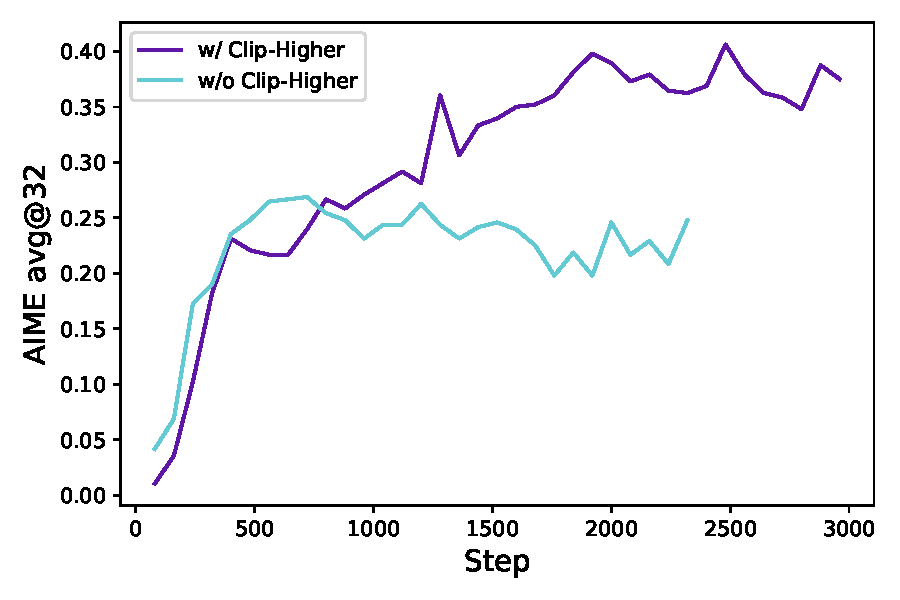
\includegraphics[width=\textwidth]{figures/3.1.2.pdf}
        \caption{Accuracies on AIME.}
        \label{fig:clighigh_acc}
    \end{subfigure}
    \hfill
    \begin{subfigure}{0.49\textwidth}
        \centering
        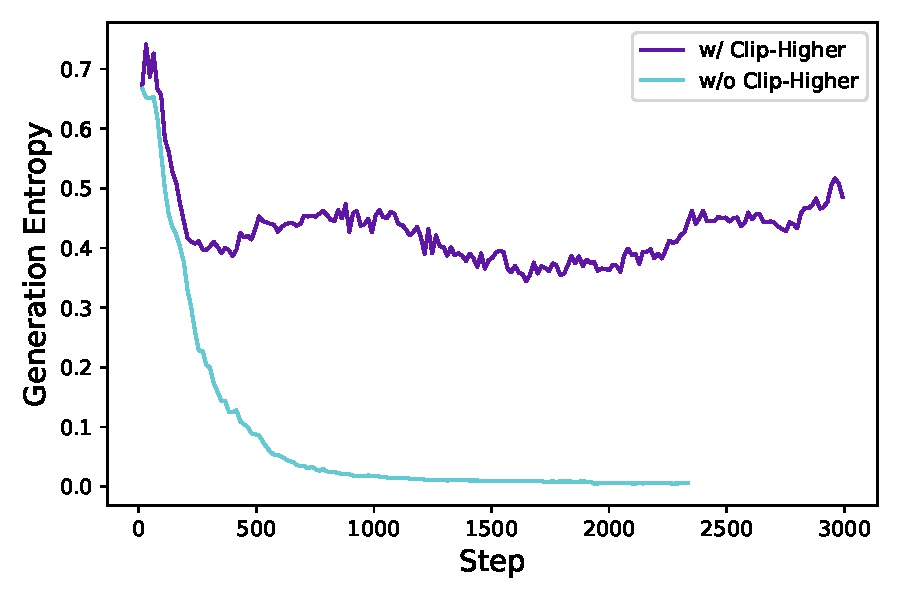
\includegraphics[width=\textwidth]{figures/3.1.1.pdf}
        \caption{Entropy of actor model.}
        \label{fig:cliphigh_entropy}
    \end{subfigure}
    \caption{The accuracy on the AIME test set and the entropy of the actor model's generated probabilities during the RL training process, both before and after applying \textbf{Clip-Higher} strategy.}
    \label{fig:clip_high}
\end{figure}


\subsection{Removing KL Divergence}
\label{sec:removekl}
The KL penalty term is used to regulate the
divergence between the online policy and the frozen reference policy. 
In the RLHF scenario~\cite{NEURIPS2022_b1efde53}, the goal of RL is to align the model behavior without diverging too far from the initial model.
However, during training the long-CoT reasoning model, the model distribution can diverge significantly from the initial model, thus this restriction is not necessary. Therefore, we will exclude the KL term from our proposed algorithm.

\subsection{Rule-based Reward Modeling}
The use of reward model usually suffers from the reward hacking problem~\cite{amodei2016concreteproblemsaisafety,
everitt2017reinforcementlearningcorruptedreward,
google2020specialgaming,
everitt2021rewardtamperingproblemssolutions,
gao2022scalinglawsrewardmodel,weng2024rewardhack}.
Instead, we directly use the final accuracy of a verifiable task as the outcome reward, computed using the following rule:
\begin{equation}
    R(\hat{y}, y) = 
    \begin{cases} 
    1, & \texttt{is\_equivalent}(\hat{y}, y) \\
    -1, & \text{otherwise} 
    \end{cases}
\end{equation}
where $y$ is the ground-truth answer and $\hat{y}$ is the predicted answer.
This is proved to be an effective approach to activating the base model's reasoning capability, as shown in multiple domains such as automated theorem proving~\cite{polu2020generativelanguagemodelingautomated,trinh2024solving,google2024alphageometry,google2024alphaproofandalphageometry}, computer programming~\cite{le2022coderl,shinn2023reflexionlanguageagentsverbal,chen2023teachinglargelanguagemodels,gehring2025rlefgroundingcodellms}, and mathematics competition~\cite{guo2025deepseek}.


\section{DAPO}
\label{sec:method}

We propose the \textbf{D}ecouple Clip and \textbf{D}ynamic s\textbf{A}mpling \textbf{P}olicy \textbf{O}ptimization (DAPO) algorithm. DAPO samples a group of outputs $\{o_i\}_{i=1}^G$ for each question $q$ paired with the answer $a$, and optimizes the policy via the following objective:
\begin{equation}
\begin{aligned}
\mathcal{J}_{\text{DAPO}}(\theta) =\quad& \mathbb{E}_{(q,a)\sim \mathcal{D}, \{o_i\}_{i=1}^G\sim \pi_{\theta_\text{old}}(\cdot\mid q)}\\&
\Bigg[\frac{1}{\sum_{i=1}^{G}|o_i|}\sum_{i=1}^{G}\sum_{t=1}^{|o_i|} 
\min \Big( r_{i,t}(\theta) \hat{A}_{i,t},  
\ \text{clip} \Big( r_{i,t}(\theta), 1 - {\varepsilon_{\text{low}}}, 1 + {\varepsilon_{\text{high}}} \Big) \hat{A}_{i,t} \Big) \Bigg]
\\
\text{s.t.}\quad& 0< \Big|\{o_i\mid\texttt{is\_equivalent}(a,o_i)\}\Big|< G,
\label{eq:dapoloss}
\end{aligned}
\end{equation}
where
\begin{equation}
    r_{i,t}(\theta)=\frac{\pi_{\theta}(o_{i,t} \mid q, o_{i,<t})}{\pi_{\theta_{\text{old}}}(o_{i,t} \mid q,o_{i,<t})},\quad\hat{A}_{i,t} = \frac{R_i - \text{mean}(\{R_i\}_{i=1}^G)}{\text{std}(\{R_i\}_{i=1}^G)}.
\label{eq:advantage_calculation}
\end{equation}
The full algorithm can be found in Algorithm~\ref{algo:dapo}. In this section, we will introduce the key techniques associated with DAPO.

\subsection{Raise the Ceiling: Clip-Higher}
\label{sec:cliphigher}

In our initial experiments using naive PPO~\cite{schulman2017proximal} or GRPO~\cite{deepseekmath}, we observed the entropy collapse phenomenon: the entropy of the policy decreases quickly as training progresses (\Cref{fig:cliphigh_entropy}). The sampled responses of certain groups tend to be nearly identical. This indicates limited exploration and early deterministic policy, which can hinder the scaling process. 

We propose the \textbf{Clip-Higher} strategy to address this issue. Clipping over the importance sampling ratio is introduced in Clipped Proximal Policy Optimization (PPO-Clip)~\cite{schulman2017proximal} to restrict the trust region and enhance the stability of RL. 
We identify that the upper clip can restrict the exploration of the policy. In this case, it is much easier to make an `exploitation token' more probable, than to uplift the probability of an unlikely `exploration token'.

Concretely, when $\varepsilon = 0.2$ (the default value of most algorithms), consider two actions with probabilities $\pi_{\theta_{\text{old}}}(o_i \mid q) = 0.01$ and $0.9$. The maximum possible updated probabilities $\pi_{\theta}(o_i \mid q)$ are $0.012$ and $1.08$, respectively. 
This implies that for tokens with a higher probability (\eg, 0.9) is less constrained. Conversely, for low-probability tokens, achieving a non-trivial increase in probability is considerably more challenging.
Empirically, we also observe that the maximum probability of clipped tokens is approximately $\pi_{\theta}(o_i \mid q) < 0.2$ (\Cref{fig:max_prob_clipped}). This finding supports our analysis that the upper clipping threshold indeed restricts the probability increase of low-probability tokens, thereby potentially constraining the diversity of the system.

Adhering to the \textbf{Clip-Higher} strategy, we decouple the lower and higher clipping range as $\varepsilon_\text{low}$ and $\varepsilon_\text{high}$, as highlighted in Equation~\ref{eq:dapoloss_clip_higher}:
\begin{equation}
\begin{aligned}
\mathcal{J}_{\text{DAPO}}(\theta) = \quad&\mathbb{E}_{(q,a)\sim\mathcal{D}, \{o_i\}_{i=1}^G\sim \pi_{\theta_\text{old}}(\cdot\mid q)}\\&
\Bigg[\frac{1}{\sum_{i=1}^{G}|o_i|}\sum_{i=1}^{G}\sum_{t=1}^{|o_i|} 
\min \Big( r_{i,t}(\theta) \hat{A}_{i,t},  
\ \text{clip} \Big( r_{i,t}(\theta), 1 - {\color{red}\varepsilon_{\text{low}}}, 1 + {\color{red}\varepsilon_{\text{high}}} \Big) \hat{A}_{i,t} \Big) \Bigg]\\
\text{s.t.}\quad& 0< \Big|\{o_i\mid\texttt{is\_equivalent}(a,o_i)\}\Big|< G.
\label{eq:dapoloss_clip_higher}
\end{aligned}
\end{equation}
We increase the value of \( \varepsilon_{\text{high}} \) to leave more room for the increase of low-probability tokens. As shown in \Cref{fig:clip_high}, this adjustment effectively enhances the policy's entropy and facilitates the generation of more diverse samples.
We opt to keep \( \varepsilon_{\text{low}} \) relatively small, because increasing it will suppress the probability of these tokens to $0$, resulting in the collapse of the sampling space.

% \begin{figure}[h]
%     \centering
%     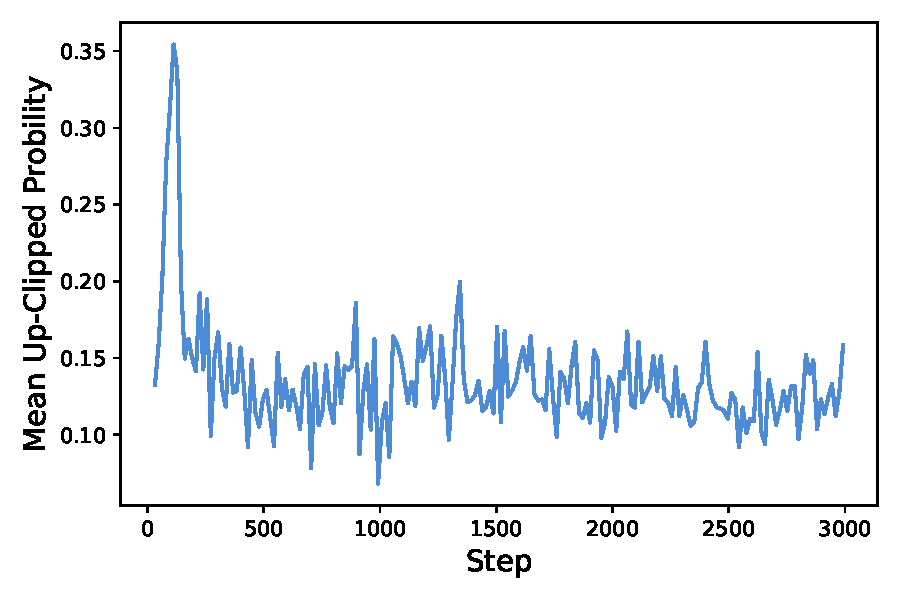
\includegraphics[width=0.5\linewidth]{figures/3.1.3.pdf}
%     \caption{Maximum clipped probabilities.}
%     \label{fig:max_prob_clipped}
% \end{figure}

% \begin{figure}[h]
%     \centering
%     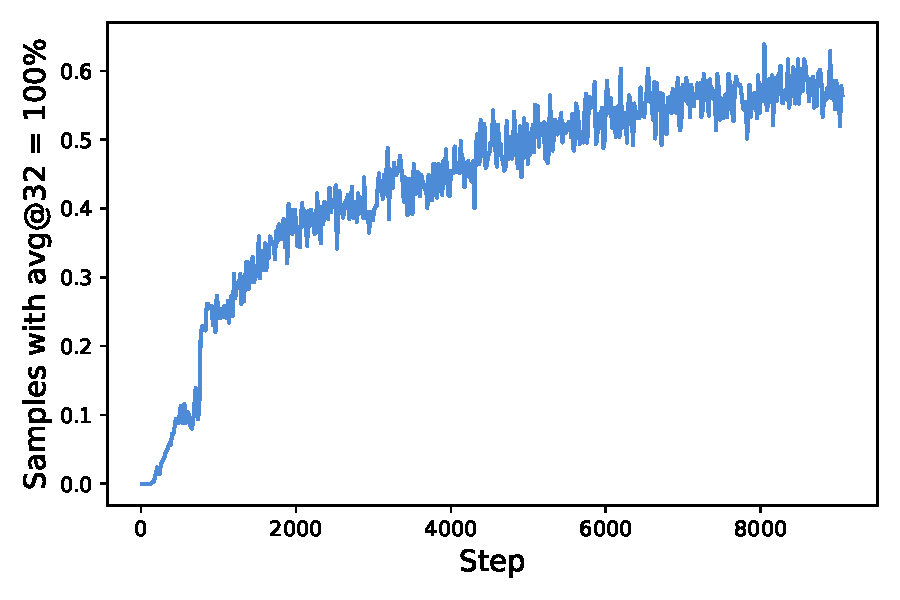
\includegraphics[width=0.5\textwidth]{figures/3.2.1.pdf}
%     \caption{The proportion of samples with an accuracy of 1 during the RL training process.}
%     \label{fig:num_samples_eq_1}
% \end{figure}

\begin{figure}
    \centering
    \begin{subfigure}{0.49\textwidth}
        \centering
        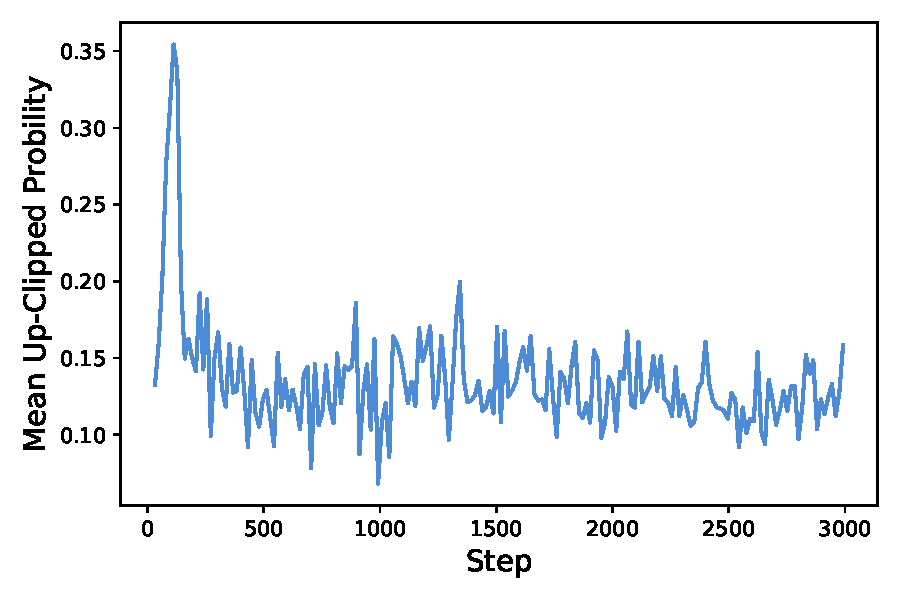
\includegraphics[width=\textwidth]{figures/3.1.3.pdf}
        \caption{Maximum clipped probabilities.}
        \label{fig:max_prob_clipped}
    \end{subfigure}
    \hfill
    \begin{subfigure}{0.49\textwidth}
        \centering
        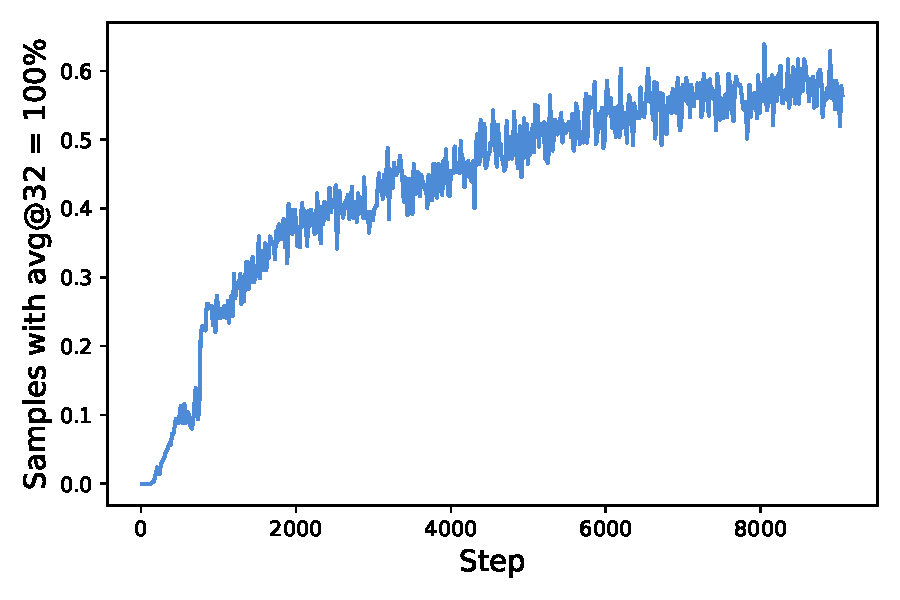
\includegraphics[width=\textwidth]{figures/3.2.1.pdf}
    \caption{The proportion of samples with an accuracy of 1.}
    \label{fig:num_samples_eq_1}
    \end{subfigure}
    
    \caption{The entropy of the probability distribution of the actor model, as well as the changes in response length.}
    \label{fig:3212}
\end{figure}

\subsection{The More the Merrier: Dynamic Sampling}
\label{sec:gradientkeeping}

Existing RL algorithm suffers from the gradient-decreasing problem when some prompts have accuracy equal to 1. For example for GRPO, if all outputs $\{o_i\}_{i=1}^G$ of a particular prompt are correct and receive the same reward 1, the resulting advantage for this group is \textit{zero}. A zero advantage results in no gradients for policy updates, thereby reducing sample efficiency. Empirically, the number of samples with accuracy equal to 1 continues to increase, as shown in \Cref{fig:num_samples_eq_1}. This means that the effective number of prompts in each batch keeps decreasing, which can lead to larger variance in gradient and dampens the gradient signals for model training.

To this end, we propose to \textbf{over-sample and filter out prompts with the accuracy equal to 1 and 0} illustrated in Equation~\ref{eq:dapoloss_oversample_filter}, leaving all prompts in the batch with effective gradients and keeping a consistent number of prompts. Before training, we keep sampling until the batch is fully filled with samples whose accuracy is neither 0 nor 1.

\begin{equation}
\begin{aligned}
\mathcal{J}_{\text{DAPO}}(\theta) =\quad& \mathbb{E}_{(q,a)\sim \mathcal{D}, \{o_i\}_{i=1}^G\sim \pi_{\theta_\text{old}}(\cdot\mid q)}\\&
\Bigg[\frac{1}{\sum_{i=1}^{G}|o_i|}\sum_{i=1}^{G}\sum_{t=1}^{|o_i|} 
\min \Big( r_{i,t}(\theta) \hat{A}_{i,t},  
\ \text{clip} \Big( r_{i,t}(\theta), 1 - {\varepsilon_{\text{low}}}, 1 + {\varepsilon_{\text{high}}} \Big) \hat{A}_{i,t} \Big) \Bigg]
\\
\text{s.t.}\quad& {\color{red}0< \Big|\{o_i\mid\texttt{is\_equivalent}(a,o_i)\}\Big|< G}.
\label{eq:dapoloss_oversample_filter}
\end{aligned}
\end{equation}

Note that this strategy does not necessarily impede training efficiency, because the generation time is typically dominated by the generation of long-tail samples if the RL system is synchronized and the generation stage is not pipelined. Besides, we find that with dynamic sampling the experiment achieves the same performance faster as shown in~\Cref{fig:afos_compare}.

% Generally, our strategy serves as a filter that screens every group of outputs and discards those rewarded with minimum or maximum scores, as these extreme samples are more likely to cluster and produce zero gradients. 
% However, a straightforward filtering approach can undermine training stability because the proportion of extreme samples varies across different batches, resulting in inconsistent numbers of useful samples at each training step. 
% To address this issue, we employ an up-sampling strategy for useful responses until the batch is fully filled. 
% Specifically, we repeat the sampling process for each prompt $q$, and subsequently discard extreme samples until the remaining samples fill the original batch size.


\subsection{Rebalancing Act: Token-Level Policy Gradient Loss}
\label{sec:tokenlevel}

The original GRPO algorithm employs a sample-level loss calculation, which involves first averaging the losses by token within each sample and then aggregating the losses across samples. In this approach, each sample is assigned an equal weight in the final loss computation. However, we find that this method of loss reduction introduces several challenges in the context of long-CoT RL scenarios.

Since all samples are assigned the same weight in the loss calculation,  tokens within longer responses (which contain more tokens) may have a disproportionately lower contribution to the overall loss, which can lead to two adverse effects.
First, for high-quality long samples, this effect can impede the model's ability to learn reasoning-relevant patterns within them.
Second, we observe that excessively long samples often exhibit low-quality patterns such as gibberish and repetitive words. Thus, sample-level loss calculation, due to its inability to effectively penalize those undesirable patterns in long samples, leads to an unhealthy increase in entropy and response length, as shown in 
\Cref{fig:token_loss_entropy} and \Cref{fig:token_loss_length}.

\begin{figure}
    \centering
    \begin{subfigure}{0.49\textwidth}
        \centering
        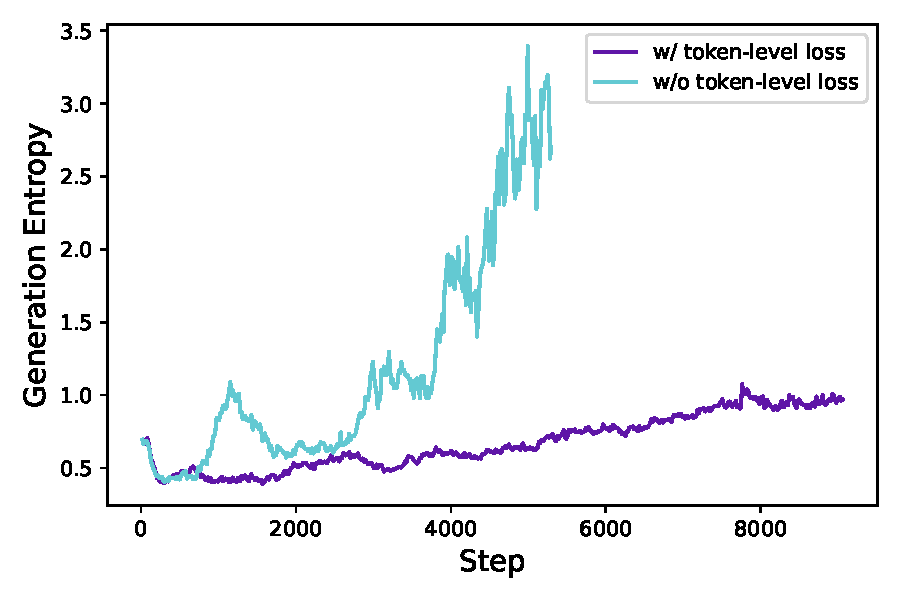
\includegraphics[width=\textwidth]{figures/3.3.1.pdf}
        \caption{Entropy of actor model's generation probabilities.}
        \label{fig:token_loss_entropy}
    \end{subfigure}
    \hfill
    \begin{subfigure}{0.49\textwidth}
        \centering
        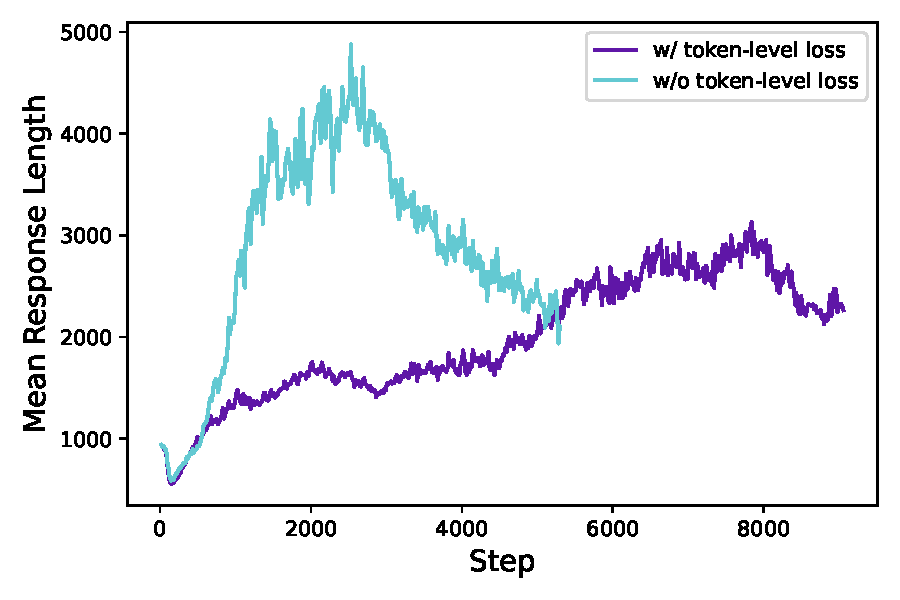
\includegraphics[width=\textwidth]{figures/3.3.2.pdf}
        \caption{Average length of actor model-generated responses}
        \label{fig:token_loss_length}
    \end{subfigure}
    
    \caption{The entropy of the probability distribution of the actor model, as well as the changes in response length.}
    \label{fig:3212}
\end{figure}

We introduce a \textbf{Token-level Policy Gradient Loss} in the long-CoT RL scenario to address the above limitations:
\begin{equation}
\begin{aligned}
\mathcal{J}_{\text{DAPO}}(\theta) = \quad&\mathbb{E}_{(q,a)\sim \mathcal{D}, \{o_i\}_{i=1}^G\sim \pi_{\theta_\text{old}}(\cdot\mid q)}\\&
\Bigg[\frac{1}{\color{red}\sum_{i=1}^{G}|o_i|}{\color{red}\sum_{i=1}^{G}\sum_{t=1}^{|o_i|}} 
\min \Big( r_{i,t}(\theta) \hat{A}_{i,t},  
\ \text{clip} \Big( r_{i,t}(\theta), 1 - {\varepsilon_{\text{low}}}, 1 + {\varepsilon_{\text{high}}} \Big) \hat{A}_{i,t} \Big) \Bigg],\\
\text{s.t.}\quad& 0< \Big|\{o_i\mid\texttt{is\_equivalent}(a,o_i)\}\Big|< G.
\label{eq:dapoloss_token_level_pg_loss}
\end{aligned}
\end{equation}
% Formally, let \( o_i \) denote a response and \( o_{i,t} \) represent the \( t \)-th token in \( o_i \), with the total number of tokens in \( o_i \) given by \( |o_i| \).
In this setting, longer sequences can have more influence on the overall gradient update compared to shorter sequences. 
Moreover, from the perspective of individual tokens, if a particular generation pattern can lead to an increase or decrease in reward, it will be equally prompted or suppressed, regardless of the length of the response in which it appears.
% The new objective function of GRPO can then be expressed as:
% \begin{equation}
% \mathcal{J}(\theta) = \mathbb{E}_{q\sim P(Q), \{o_i\}_{i=1}^G\sim \pi_{\theta_\text{old}}(O\mid q)}
% \Bigg[\frac{1}{\sum_{i=1}^{G}|o_i|}\sum_{i=1}^{G}\sum_{t=1}^{|o_i|} 
% \min \Big( r_{i,t}(\theta) \hat{A}_{i,t},  
% \ \text{clip} \Big( r_{i,t}(\theta), 1 - \varepsilon_{\text{low}}, 1 + \varepsilon_{\text{high}} \Big) \hat{A}_{i,t} \Big) \Bigg].
% \label{eq:token-level-grpo}
% \end{equation}

% \paragraph{Removal of KL Penalty} The KL penalty was originally introduced in reinforcement learning to regulate the divergence between the online policy and the frozen reference policy. In conventional RLHF settings, the goal during the RL phase is to optimize model alignment while preserving the SFT model generation patterns. However, during training of the reasoning model, the output distribution diverges significantly from base model. In this context, the KL regularization term may instead hinder training progress. Our experiments demonstrate that removing the KL penalty from the loss function leads to improved performance.

% \begin{equation}
% \mathcal{J}_{GRPO}(\theta) =
% \frac{1}{G\sum_{i=1}^{G}{|o_i|}} \sum_{i=1}^{G} \sum_{t=1}^{|o_i|} 
% \min \Bigg[
% \frac{\pi_{\theta} (o_{i,t} \mid q, o_{i,<t})}{\pi_{\theta_{old}} (o_{i,t} \mid q, o_{i,<t})} \hat{A}_{i,t}, 
% \operatorname{clip} \Bigg( 
% \frac{\pi_{\theta} (o_{i,t} \mid q, o_{i,<t})}{\pi_{\theta_{old}} (o_{i,t} \mid q, o_{i,<t})}, 1 - \varepsilon, 1 + \varepsilon 
% \Bigg) \hat{A}_{i,t}\Bigg]
% \label{eq:token-level-grpo-our}
% \end{equation}


\subsection{Hide and Seek: Overlong Reward Shaping}
\label{sec:overlong}

In RL training, we typically set a maximum length for generation, with overlong samples truncated accordingly. We find that improper reward shaping for truncated samples can introduce reward noise and significantly disrupt the training process.

By default, we assign a punitive reward to truncated samples.
This approach may introduce noise into the training process, as a sound reasoning process can be penalized solely due to its excessive length. Such penalties can potentially confuse the model regarding the validity of its reasoning process.

\vspace{5pt}
To investigate the impact of this reward noise, we first apply an \textbf{Overlong Filtering} strategy which masks the loss of truncated samples. We find that this approach significantly stabilizes training and enhances performance, as demonstrated in \Cref{fig:overlong_shaping}.

\begin{figure}[t]
    \centering
    \begin{subfigure}{0.49\textwidth}
        \centering
        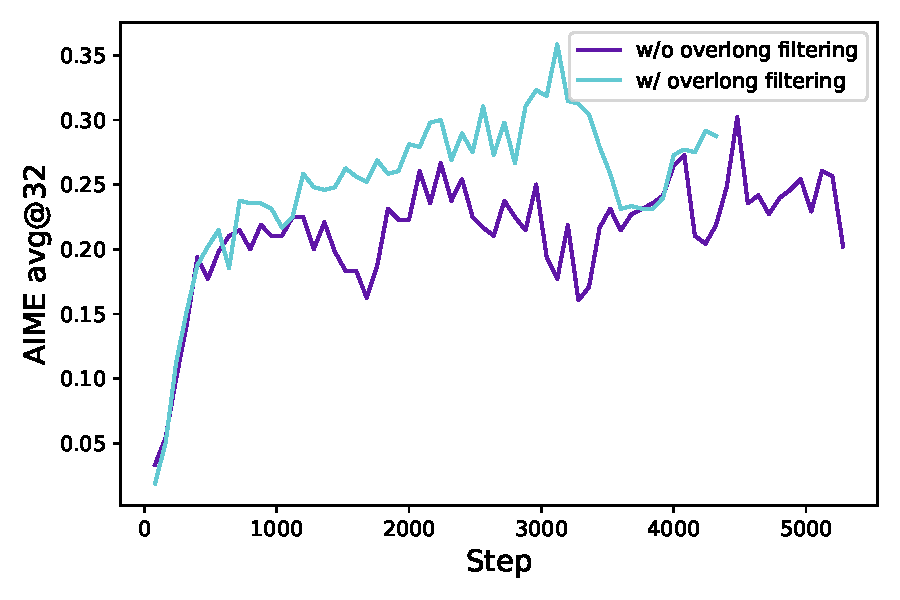
\includegraphics[width=\textwidth]{figures/3.4.1.pdf}
        \caption{Performance on AIME.}
        \label{fig:overlong_acc}
    \end{subfigure}
    \hfill
    \begin{subfigure}{0.49\textwidth}
        \centering
        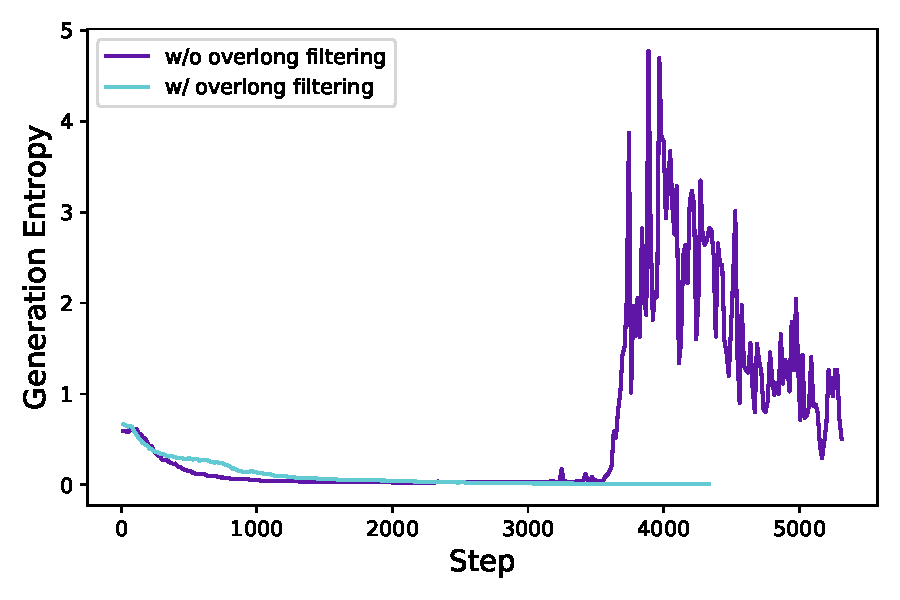
\includegraphics[width=\textwidth]{figures/3.4.2.pdf}
        \caption{Entropy of actor model.}
        \label{fig:overlong_entropy}
    \end{subfigure}
    \caption{The accuracy of the actor model on AIME and the entropy of its generation probabilities, both before and after applying \textbf{Overlong Reward Shaping} strategy.}
    \label{fig:overlong_shaping}
\end{figure}

\setcounter{table}{0}
\begin{table}[h]
    \centering
    \begin{tabular}{@{}p{1.0\textwidth}@{}} 
        \toprule 
        \textbf{Algorithm 1} \; \textbf{DAPO}: \textbf{D}ecoupled Clip and \textbf{D}ynamic s\textbf{A}mpling \textbf{P}olicy \textbf{O}ptimization \\
        \midrule 
        \textbf{Input} initial policy model $\pi_\theta$; reawrd model $R$; task prompts $\mathcal{D}$; hyperparameters $\varepsilon_\mathtt{low}, \varepsilon_\mathtt{high}$ \\
        \;1: \textbf{for} step = 1,...,M \textbf{do} \\
        \;2: \;\;\; Sample a batch $\mathcal{D}_b$ from $\mathcal{D}$ \\
        \;3: \;\;\; Update the old policy model $\pi_{\theta_{old}} \leftarrow \pi_\theta$\\
        \;4: \;\;\; Sample \textit{G} outputs $\{o_i\}_{i=1}^{G} \sim \pi_{\theta_{\text{old}}}(\cdot | q)$ for each question $q \in \mathcal{D}_b$ \\
        \;5: \;\;\; Compute rewards $\{r_i\}_{i=1}^{G}$ for each sampled output $o_i$ by running $R$ \\
        \;6: \;\;\; Filter out $o_i$ and add the remaining to the dynamic sampling buffer (\textbf{Dynamic Sampling} \Cref{eq:dapoloss_oversample_filter})\\
        \;7: \;\;\; \textbf{if} buffer size $n_b<N$: \\
        \;8: \;\;\;\;\;\;\;\; \textbf{continue} \\
            \;9: \;\;\; For each $o_i$ in the buffer, compute $\hat{A}_{i,t}$ for the \textit{t}-th token of $o_i$ (\Cref{eq:advantage_calculation}) \\
        \;10: \;\; \textbf{for} iteration = 1, ..., $\mu$ \textbf{do}\\
        \;11: \;\;\;\;\;\;\; Update the policy model $\pi_\theta$ by maximizing the DAPO objective (\Cref{eq:dapoloss})\\
        \textbf{Output} $\pi_\theta$\\
        \bottomrule
    \end{tabular}
    \captionsetup{labelformat=empty}
    \caption{}
    \label{algo:dapo}
\end{table}
\vspace{-10pt}

Furthermore, we propose \textbf{Soft Overlong Punishment} (Equation~\ref{eq:soft_punish}), a length-aware penalty mechanism designed to shape the reward for truncated samples. 
Specifically, when the response length exceeds the predefined maximum value, we define a punishment interval. Within this interval, the longer the response, the greater the punishment it receives.
%Specifically, beyond the predefined maximum length, we introduce an additional cache range for continuous soft punish where longer responses will be punished more. 
This penalty is added to the original rule-based correctness reward, thereby signaling to the model to avoid excessively long responses.


\begin{equation}
R_{\text{length}}(y) =
\begin{cases}
0, & |y| \le L_{\text{max}} - L_{\text{cache}} \\
\frac{(L_{\text{max}} - L_{\text{cache}}) - |y|}{L_{\text{cache}}}, & L_{\text{max}} - L_{\text{cache}}<|y|\le L_{\text{max}} \\
-1, & L_{\text{max}} < |y|
\end{cases}
\label{eq:soft_punish}
\end{equation}



% Therefore, we propose two improvements, \textbf{Overlong Mask} and \textbf{Overlong Punish}, to address this issue:
% \begin{itemize}
%     \item \textbf{Overlong Mask}: We exclude truncated overlong samples by masking them from group normalization calculations, which effectively reduces reward noise. 
%     However, since the model remains entirely unaware of samples that do not contribute gradient signals, it leads to an accumulation of excessively long responses in later training stages, ultimately reducing training efficiency.
%     \item \textbf{Overlong Punish}: 
% \end{itemize}

\subsection{Dataset Transformation}
\label{sec:dataprocess}

Our dataset is sourced from the AoPS\footnote{https://artofproblemsolving.com/} website and official competition homepages through a combination of web scraping and manual annotation.
The answers of math dataset typically come in a variety of formats, such as expression, formula and number, which makes it challenging to design comprehensive rules to parse them.
To provide accurate reward signals using rules and minimize errors introduced by formula parsers, inspired by AIME, we select and transform the answers into integers, which are easy to parse.
For example, if the original answer is expressed in the form of \( \frac{a + \sqrt{b}}{c} \), we instruct the LLM to modify the question so that the expected answer becomes \( a + b + c \).
After selection and transformation, we obtained the \textbf{\method-Math-17K} dataset, which consists of 17K prompts, each paired with an integer as the answer.
% Such an answer format proves to be difficult to hack.



% \newpage
\section{Experiments}

% \subsection{Setup}
\paragraph{Setup}
We employ BERT~\citep{devlin-etal-2019-bert} as the commonly-used base model in previous works. In addition, we extend our evaluation to RoBERTa~\citep{liu2019roberta} and GPT-2~\citep{radford2019language} for a more comprehensive analysis.

\paragraph{Datasets} We evaluate our debiasing framework on three NLP datasets including 
MNLI~\citep{williams-etal-2018-broad}, 
paraphrase identification using Quora question pairs (QQP)~\citep{sharma2019natural}, and
relation extraction using gene-phenotype relation (PGR)~\citep{sousa-etal-2019-silver}. 
% We use their corresponding \textbf{In-Domain Test Sets} for evaluation.
These datasets are used for {\em in-domain} (ID) evaluation.

\paragraph{Stress Test Sets} We assess the robustness of models against spurious correlations using ``stress test sets,'' specifically designed with hard examples to challenge models. 
% We test if models are robust to spurious correlations with \textit{stress test sets} which contain hard examples created to fool models. 
We use the stress test set for MNLI from~\citep{naik-etal-2018-stress}, and
use the same approach to generate the stress test set for QQP.
% following the same label preserving rules from~\citep{naik-etal-2018-stress}. 
For PGR, the label-preserving rules from previous tasks do not apply due to the nature of this dataset.
% the above rules are not be applicable since it doesn't align with the nature of the task. However, 
However, given the long-tail distribution of entity appearances, we create a stress test set for PGR by selecting test examples in which both entities appear less than five times in the training set.

\paragraph{OOD Test Sets} We assess the performance of models on existing out-of-distribution (OOD) test sets, which serve as another challenge benchmark. For MNLI, we use HANS~\citep{mccoy-etal-2019-right}, which is designed to test models' capabilities against lexical and syntactic heuristics in data. For QQP, we employ the PAWS dataset~\citep{zhang-etal-2019-paws}, which focuses on paraphrase identification in cases of high lexical and surface-level similarity between question pairs.

\paragraph{Transfer Test Sets} We evaluate the performance of models in maintaining strong transferability across datasets. We use SNLI~\citep{bowman-etal-2015-large} and MRPC~\citep{dolan-brockett-2005-automatically} as the transfer set for MNLI and QQP, respectively. 
% \paragraph{Probing set}
% Previous work~\citep{mendelson-belinkov-2021-debiasing} discovered that debiased models can be still biased. We use the probing set to probe if there still exists dataset bias in our model.

\begin{table*}
\tiny
\centering
% \setlength{\tabcolsep}{3.9pt}
% \renewcommand{\arraystretch}{0.9} 
\begin{tabular}{l|cccc|cccc|cc|cccc}
\toprule
\multirow{2}{2em}{\textbf{Model}} & \multicolumn{4}{c|}{\textbf{MNLI} (Acc.)} & \multicolumn{4}{c|}{\textbf{QQP} (F1)} & \multicolumn{2}{c|}{\textbf{PGR} (F1)} & \multicolumn{4}{c}{\textbf{Avg.}}\\
               & ID   & Stress & OOD & Transfer & ID & Stress & OOD & Transfer & ID & Stress & ID & Stress & OOD & Transfer \\ 
    \toprule
    \textbf{\FT}        & 84.3 & 61.7 & 59.7 & 78.7 & 88.6 & 63.3 & 47.7 & 65.1 & 64.3 & 55.2 & 79.1 & 60.1 & 53.7 & 71.9 \\ 
    \midrule
    \textbf{\MASK}      & 83.5 & 59.7 & 59.7 & 78.3 & 88.1 & 64.6 & 50.3 & 68.5 & 64.1 & 51.7 & 78.6 & 58.7 & 55.0 & 73.4 \\ 
    \textbf{\KW}        & 84.0 & 60.9 & 60.2 & 78.4 & 88.8 & 65.1 & 51.2 & 69.6 & 64.3 & 51.8 & 79.0 & 59.3 & 55.7 & 74.0 \\ 
    \textbf{\ETE}       & 83.4 & 61.3 & 62.3 & 77.5 & 88.5 & 64.5 & 51.4 & 70.5 & 63.0 & 53.6 & 78.3 & 59.8 & 56.8 & 74.0 \\
    \textbf{LSWC}       & 80.7 & 59.4 & 59.3 & 77.7 & 87.1 & 65.8 & 49.6 & 70.0 & 63.3 & 52.8 & 77.0 & 59.3 & 54.5 & 73.8 \\ 
    \textbf{\IE}        & 84.1 & 61.8 & 62.7 & 78.1 & 87.6 & 63.5 & 53.0 & 68.3 & 64.2 & 54.9 & 78.6 & 60.1 & 57.9 & 73.2 \\
    \textbf{\READ}      & 80.8 & 61.5 & 63.4 & 75.1 & 87.0 & 66.7 & 53.6 & 68.2 & 63.0 & 54.4 & 76.9 & 60.9 & 58.5 & 71.7 \\ 
    \midrule
    \textbf{\OursPoe}   & 84.6 & 64.3 & 64.3 & 79.5 & 88.8 & 71.0 & 53.9 & 70.4 & 64.9 & 55.9 & 79.4 & 63.7 & 59.1 & \underline{75.0} \\ 
    \textbf{\OursFocal} & \underline{84.9} & \underline{64.8} & \underline{64.3} & \underline{79.3} & \underline{89.5} & \underline{71.3} & \underline{54.9} & \underline{70.7} & \underline{65.4} & \underline{56.5} & \underline{79.9} & \underline{64.2} & \underline{59.6} & \underline{75.0} \\
    \textbf{\OursCL}    & \textbf{85.1} & \textbf{65.4} & \textbf{64.9} & \textbf{79.6} & \textbf{90.4} & \textbf{72.0} & \textbf{56.0} & \textbf{72.4} & \textbf{65.9} & \textbf{56.6} & \textbf{80.5} & \textbf{64.7} & \textbf{60.5} & \textbf{76.0} \\ 
    \bottomrule
  \end{tabular}
  \caption{Experimental results on three datasets averaged across three architectures. Results for each architecture are shown in Table~\ref{tab:bert}-\ref{tab:gpt2} in Appendix. The best performance is in \textbf{bold} and the second best is \underline{underlined}.}
  \label{tab:main}
\end{table*}


\begin{table*}
\small
\centering
\begin{tabular}{l|cccc}
\toprule
\multirow{2}{*}{\textbf{Model}} & \multicolumn{4}{c}{\textbf{Avg.}}\\
                & ID & Stress & OOD & Transfer \\ 
    \midrule
    \textbf{\FT}        & 79.1 & 60.1 & 53.7 & 71.9 \\ 
    \midrule
    \textbf{\ETE}       & 78.3 & 59.8 & 56.8 & 74.0 \\
    \textbf{\MASK}      & 78.6 & 58.7 & 55.0 & 73.4 \\ 
    \textbf{LSWC}       & 77.0 & 59.3 & 54.5 & 73.8 \\ 
    \textbf{\IE}        & 78.6 & 60.1 & 57.9 & 73.2 \\
    \textbf{\KW}        & 79.0 & 59.3 & 55.7 & 74.0 \\ 
    \textbf{\READ}      & 76.9 & 60.9 & 58.5 & 71.7 \\ 
    \midrule
    \textbf{\OursPoe}   & 79.4 & 63.7 & 59.1 & \underline{75.0} \\ 
    \textbf{\OursFocal} & \underline{79.9} & \underline{64.2} & \underline{59.6} & \underline{75.0} \\
    \textbf{\OursCL}    & \textbf{80.5} & \textbf{64.7} & \textbf{60.5} & \textbf{76.0} \\ 
    \bottomrule
  \end{tabular}
\end{table*}


\paragraph{Baselines} 
We consider the following baselines:
\vspace{-5pt}
\begin{itemize}
    \itemsep-2pt
    \itemindent-10pt
    \item \textbf{\FT} standard finetuning without debiasing based on the base model used. 
    % \item \textbf{Rubi}~\citep{cadene2019rubi}, which models the bias of input texts to re-weight the prediction loss in text-image classification. In our experiments, we replace the image encoder in Rubi with a text encoder.
    \item \textbf{\ETE}~\citep{karimi-mahabadi-etal-2020-end}, which trains a biased model on the hypothesis only and trains a robust model using Product of Experts (PoE)~\citep{10.1162/089976602760128018}.
    \item \textbf{\MASK}~\citep{meissner-etal-2022-debiasing}, which first trains a weak learner and then prunes the robust model using PoE. %odel.
    \item \textbf{\KW}~\citep{gao-etal-2022-kernel}, which learns isotropic sentence embeddings using Nystr\"{o}m kernel approximation~\citep{Xu_Jin_Shen_Zhu_2015} method, achieving disentangled correlation between robust and spurious embeddings.
    \item \textbf{LWBC}~\citep{kim2022learning}, which learns a debiased model from a commitee of biased model obtained from subsets of data.
    \item \textbf{\IE}~\citep{du-etal-2023-towards}, which mitigates dataset biases with an ensemble of random biased induction forest; the model induces a set of biased features and then purifies the biased features using information entropy\footnote{While this method does not have a publicly released code, we tried our best to reproduce their approach and results with a few points lower than reported.}.
    \item \textbf{\READ}~\citep{wang-etal-2023-robust}, which assumes that spuriousness comes from the attention
    % of \texttt{[CLS]} over other tokens 
    and proposes to do deep ensemble of main and biased model at the attention level to learn robust feature interaction.
\end{itemize}




% \input{sections/050discussion}
% \section{Related Work}

\subsection{Reasoning Models}

\subsection{Reinforcement Learning}

\section{Conclusion}

In this paper, we release a fully open-sourced system for large-scale LLM RL, including algorithm, code infrastructure, and dataset. The system achieves state-of-the-art large-scale LLM RL performance (AIME 50 using Qwen-32B pretrained model). We propose the \textbf{D}ecoupled Clip and \textbf{D}ynamic s\textbf{A}mpling \textbf{P}olicy \textbf{O}ptimization (\textbf{DAPO}) algorithm, and introduce 4 key techniques to make RL powerfully effective and efficient in the long-CoT RL scenario.
Additionally, by open-sourcing the training code and dataset, we provide the broader research community and society with practical access to a scalable reinforcement learning solution, enabling all to benefit from these advancements. 

\newpage

\section*{Contributions}

\textbf{Project Lead}\quad 

Qiying Yu$^{1,2,4}$

% \subsection*{Algorithm}

\textbf{Algorithm}

Qiying Yu$^{1,2,4}$, Zheng Zhang$^{1}$, Ruofei Zhu$^{1}$, Yufeng Yuan$^{1}$, Xiaochen Zuo$^{1}$, Yu Yue$^{1}$

% \subsection*{Infrastructure$^{*}$}

\textbf{Infrastructure$^{*}$}

Tiantian Fan$^{1}$, Gaohong Liu$^{1}$, Lingjun Liu$^{1}$, Xin Liu$^{1}$, Haibin Lin$^{1}$, Zhiqi Lin$^{1}$, Bole Ma$^{1}$, Guangming Sheng$^{1,3}$, Yuxuan Tong$^{1,2,4}$, Qiying Yu$^{1,2,4}$, Chi Zhang$^{1}$, Mofan Zhang$^{1}$, Wang Zhang$^{1}$, Hang Zhu$^{1}$, Jinhua Zhu$^{1}$

$^{*}$Last-Name in Alphabetical Order

% \subsection*{Dataset}

\textbf{Dataset}

Jiaze Chen$^{1}$, Jiangjie Chen$^{1,4}$, Chengyi Wang$^{1}$, Hongli Yu$^{1,2,4}$, Weinan Dai$^{1,2,4}$, Yuxuan Song$^{1,2,4}$, Xiangpeng Wei$^{1}$, Qiying Yu$^{1,2,4}$

% \subsection*{Supervision}

\textbf{Supervision}

Hao Zhou$^{2,4}$, Jingjing Liu$^{2,4}$, Wei-Ying Ma$^{2,4}$, Ya-Qin Zhang$^{2,4}$, Lin Yan$^{1,4}$, Mu Qiao$^{1,4}$, Yonghui Wu$^{1}$, Mingxuan Wang$^{1,4}$

% \subsection*{Affiliation}

\textbf{Affiliation}

% $^1$\textsf{ByteDance Seed}

% $^2$\textsf{Institute for AI Industry Research (AIR), Tsinghua University}

% $^3$\textsf{The University of Hong Kong}

% $^4$\textsf{SIA-Lab of Tsinghua AIR and ByteDance Seed}

$^1$ByteDance Seed

$^2$Institute for AI Industry Research (AIR), Tsinghua University

$^3$The University of Hong Kong

$^4$SIA-Lab of Tsinghua AIR and ByteDance Seed

\section*{Acknowledgments}

We thank Zhengyin Du, Kai Shen, Tianyang Zhan, Zhen Xiao, Renjie Zheng, Li Han, Kaihua Jiang as well as other colleagues at ByteDance for their support for the \method project.

\clearpage

\bibliographystyle{unsrt}
% \bibliographystyle{plainnat}
\bibliography{main}

\clearpage

\beginappendix

\appendix


% \vskip 0.2cm
\section{Experimental Settings}
\label{section:reproduce}

% \vskip -0.2cm
\paragraph{Supervised image classification.} For all supervised classification experiments on ImageNet-1K, we follow the training recipes from ConvNeXt \citep{convnext}.
For ConvNeXt-B and ConvNeXt-L, we use the original hyperparameters without modification.
ViT-B and ViT-L models use the same hyperparameters as ConvNeXt-B, except that for ViT-L, the beta parameters for AdamW are set to (0.9, 0.95), and the stochastic depth rates are set to 0.1 for ViT-B and 0.4 for ViT-L. 

% \vskip 0.2cm
\paragraph{Diffusion models.} We use the official implementation~\citep{dit} for training all DiT models. We find that the default learning rate is suboptimal for the models considered in this paper. To address this, we conduct a simple learning rate search with the LN models and apply the tuned learning rates directly to the DyT models. We also observe that the zero initialization negatively affects the performance of DyT models. Therefore, we retain the zero initialization for LN models but remove the zero initialization for DyT models.

% \vskip 0.2cm
\paragraph{Large Language Models.} In our implementation of LLaMA models~\citep{touvron2023llama, touvron2023llama2, dubey2024llama} with DyT, we introduce an additional learnable scalar parameter immediately after the embedding layer, before any Transformer blocks. We initialize it to the square root of the model embedding dimension $\sqrt{d}$. Without this scaling scalar, we find that the magnitudes of model activations at the beginning of training are too small, and the training struggles to progress. The issue is mitigated by incorporating a learnable scalar, and the model can converge normally. This addition of a scalar is similar to the original Transformer~\citep{vaswani2017attention} design, which uses a fixed scalar of the same value at the same position.

We train all our LLaMA models on the Pile dataset~\citep{pile}. We use the codebase from \texttt{FMS-FSDP} \citep{fms-fsdp}, which provides a default training recipe for the 7B model that closely follows the LLaMA 2 paper~\citep{touvron2023llama2}. We maintain the learning rate at the default 3e-4 for 7B and 13B and 1.5e-4 for 34B and 70B, in line with LLaMA 2.
The batch size is set to 4M tokens
and each model is trained on a total of 200B tokens.


For evaluation, we test the pretrained models on 15 zero-shot commonsense reasoning tasks from \texttt{lm-eval} \citep{eval-harness}: \texttt{anli\_r1}, \texttt{anli\_r2}, \texttt{anli\_r3}, \texttt{arc\_challenge}, \texttt{arc\_easy}, \texttt{boolq}, \texttt{hellaswag}, \texttt{openbookqa}, \texttt{piqa}, \texttt{record}, \texttt{rte}, \texttt{truthfulqa\_mc1}, \texttt{truthfulqa\_mc2}, \texttt{wic}, and \texttt{winogrande}. The selection closely follows that of OpenLLaMA~\citep{openlm2023openllama}. We report the average performance across all tasks.



% \vskip 0.2cm
\paragraph{Self-supervised learning in speech.} For both wav2vec 2.0 models, we retain the first group normalization layer from the original architecture, as it functions primarily as data normalization to handle the unnormalized input data.
We use the official implementation \citep{wav2vec2} without modifying hyperparameters for both the Base and Large models. We report the final validation loss.

% \vskip 0.2cm
\paragraph{Other tasks.} For all other tasks, MAE \citep{he2022masked}, DINO \citep{caron2021emerging}, HyenaDNA \citep{nguyen2024hyenadna} and Caduceus \citep{schiff2024caduceus}, we directly use the publicly released code \citep{mae, dino, hyena, caduceus}, without hyperparameter tuning, for both models with LN and DyT.


% \clearpage
% \newpage
% \vskip -0.2cm
\section{Hyperparameters}
\label{section:tuning}




We present additional experiments to evaluate the impact of hyperparameter tuning, specifically focusing on the learning rate and initialization of $\alpha$ for all non-LLM models. 

\paragraph{Tuning learning rate.} Table~\ref{table:tuned_lr} summarizes performance comparisons between models trained with original versus tuned learning rates. Results indicate that tuning the learning rate provides only modest performance improvements for DyT models. This suggests that the original hyperparameters, initially optimized for LN models, are already well-suited for DyT models. This observation underscores the inherent similarity between the DyT and LN models.

\begin{table}[h]
\centering
\tablestyle{7pt}{1.15}
\begin{tabular}{lcccc}
\toprule
model & LN (original) & DyT (original) & LN (tuned) & DyT (tuned)  \\
\midrule
ViT-B & 82.3\% \scriptsize{(4e-3)} & {82.5\%} \scriptsize{(4e-3)} & - & {82.8\%} \scriptsize{(6e-3)} \\
ViT-L & 83.1\% \scriptsize{(4e-3)} & {83.6\%} \scriptsize{(4e-3)} & - & - \\
ConvNeXt-B & 83.7\% \scriptsize{(4e-3)} & 83.7\% \scriptsize{(4e-3)} & - & - \\
ConvNeXt-L & 84.3\% \scriptsize{(4e-3)} & {84.4\%} \scriptsize{(4e-3)} & - & - \\
\midrule
MAE ViT-B & 83.2\% \scriptsize{(2.4e-3)} & 83.2\% \scriptsize{(2.4e-3)} & - & 83.7\% \scriptsize{(3.2e-3)} \\
MAE ViT-L & {85.5\%} \scriptsize{(2.4e-3)} & 85.4\% \scriptsize{(2.4e-3)} & - & {85.8\%} \scriptsize{(3.2e-3)} \\
DINO ViT-B (patch size 16) & 83.2\% \scriptsize{(7.5e-4)} & {83.4\%} \scriptsize{(7.5e-4)} & 83.3\% \scriptsize{(1e-3)} & - \\
DINO ViT-B (patch size 8) & 84.1\% \scriptsize{(5e-4)} & {84.5\%} \scriptsize{(5e-4)} & - & - \\
\midrule
DiT-B & 64.9 \scriptsize{(4e-4)} & {63.9} \scriptsize{(4e-4)} & - & - \\
DiT-L & {45.9} \scriptsize{(4e-4)} & 45.7 \scriptsize{(4e-4)} & - & - \\
DiT-XL & {19.9} \scriptsize{(4e-4)}  & 20.8 \scriptsize{(4e-4)} & - & - \\
\midrule
wav2vec 2.0 Base & 1.95 \scriptsize{(5e-4)} & 1.95 \scriptsize{(5e-4)} & - & {1.94} \scriptsize{(6e-4)} \\
wav2vec 2.0 Large & 1.92 \scriptsize{(3e-4)} & {1.91} \scriptsize{(3e-4)} & - & - \\
\midrule
HyenaDNA & 85.2\% \scriptsize{(6e-4)} & 85.2\% \scriptsize{(6e-4)} & - & - \\
Caduceus & 86.9\% \scriptsize{(8e-3)} & 86.9\% \scriptsize{(8e-3)} &  - & - \\
\midrule
  \end{tabular}
\caption{\textbf{Performance comparison between original and tuned learning rates for LN and DyT models.} Results show that tuning learning rates provide only modest performance improvements for DyT models, suggesting that the default hyperparameters optimized for LN models are already well-suited for DyT models. Entries marked with ``-'' indicate no performance gain over the original learning rate. The values in parentheses represent the learning rate used. 
}
\label{table:tuned_lr}
\end{table}


\paragraph{Tuning initial value of $\alpha$.} We also investigate the effects of optimizing $\alpha_0$ for DyT models, as presented in Table~\ref{table:tune_alpha}. Findings show only minor performance enhancements for select models when $\alpha_0$ is tuned, indicating that the default initial value ($\alpha_0 = 0.5$) generally achieves near-optimal performance.



\begin{table}[h]
\vskip -0.07in
\centering
\tablestyle{7pt}{1.15}
\begin{tabular}{lcccc}
\toprule
Model & LN  & DyT ($\alpha_0 = 0.5$) & DyT (tuned) \\
\midrule
ViT-B & 82.3\% & 82.5\% & 82.6\% \scriptsize{($\alpha_0 = 1.0$)} \\
ViT-L & 83.1\% & 83.6\% & - \\
ConvNeXt-B & 83.7\% & 83.7\% & - \\
ConvNeXt-L & 84.3\% & 84.4\% & - \\
\midrule
MAE ViT-B & 83.2\% & 83.2\% & 83.4\% \scriptsize{($\alpha_0 = 1.0$)} \\
MAE ViT-L & 85.5\% & 85.4\% & - \\
DINO ViT-B (patch 16) & 83.2\% & 83.4\% & - \\
DINO ViT-B (patch 8) & 84.1\% & 84.5\% & - \\
\midrule
DiT-B & 64.9 & 63.9 & - \\
DiT-L & 45.9 & 45.7 & - \\
DiT-XL & 19.9 & 20.8 & -  \\
\midrule
wav2vec 2.0 Base & 1.95 & 1.95 & - \\
wav2vec 2.0 Large & 1.92 & 1.91 & 1.90 \scriptsize{($\alpha_0 = 1.0$)} \\
\midrule
HyenaDNA & 85.2\% & 85.2\% & -  \\
Caduceus & 86.9\% & 86.9\% & - \\
\midrule
  \end{tabular}
 \caption{\textbf{Impact of tuning the $\alpha_0$ in DyT models.} Optimizing $\alpha_0$ from the default value ($\alpha_0 = 0.5$)  yields only minor performance gains for select DyT models, implying the default initialization already achieves near-optimal performance. Entries marked with ``-'' indicate no improvement over the default $\alpha_0$.
}
\label{table:tune_alpha}
\end{table}








% \clearpage
% \newpage

\section{Replacing Batch Normalization with DyT}
\label{section:batch_normalization}

We investigate the potential of replacing BN with DyT in classic ConvNets such as ResNet-50~\citep{he2016deep} and VGG19~\citep{simonyan2014very}.
Both models are trained on the ImageNet-1K dataset~\citep{deng2009imagenet} using the training recipes provided by \texttt{torchvision}. The DyT models are trained using the same hyperparameters as their BN counterparts.

\begin{table}[h]
\centering
\tablestyle{7pt}{1.15}
\begin{tabular}{lcccccc}
\toprule
model & BN & DyT \\
\midrule
ResNet-50 & 76.2\% & 68.9\% \\
VGG19   & 72.7\% & 71.0\% \\
\midrule
\end{tabular}
\caption{\textbf{ImageNet-1K classification accuracy with BN and DyT.} Replacing BN with DyT in ResNet-50 and VGG19 results in a performance drop, indicating that DyT cannot fully substitute BN in these architectures.}
\label{table:bn_ablation}
\end{table}

The results are summarized in Table~\ref{table:bn_ablation}. Replacing BN with DyT led to a noticeable drop in classification accuracy for both models. These findings indicate that DyT is struggling to fully replace BN in these classic ConvNets. We hypothesize this could be related to BN layers being more frequent in these ConvNets, where they appear once with every weight layer, but LN only appears once per several weight layers in Transformers.

\end{document}